\usepackage{graphicx}
\usepackage{subcaption}
\usepackage{float}

\section{Photometric Classification of Supernovae}
\textit{Contributors: Tarek Allam Jr., Jason D. McEwen, Michelle Lochner, Rahul
Biswas, Robert Schuhmann, Hiranya Peiris, Ren\'ee Hlo\v{z}ek and Christian Setzer} \\
\textit{Authors: Tarek Allam Jr.\footnote{tarek.allam.10@ucl.ac.uk}} \\

The aim of this investigation is to analyse the affect a particular cadence has
on ones ability to photometrically classify supernova. This investigation has been carried out by the
developers of \ttt{snmachine} who work in the Supernova Working Group under the umbrella of the Dark Energy Science
Collaboration (DESC). \ttt{snmachine} is a DESC product that is used as a photometric
classification pipeline \cite{lochner2016photometric}.

The motivation for this work comes from the desire to identify as many Supernova
as Type 1a in order to help constrain the nature of Dark Energy.
LSST will observe many more Supernova than ever before, but at a rate that is
not feasible for all of these transients to be spectroscopically followed up and
confirmed as Type 1a or not.
Thus, the ability to classify these objects photometrically will be very
important. If one can obtain a greater set of Type 1a's, an updated Hubble
digram plot can be produced and the fundamental parameters of the cosmological
model can be tested further.

In order to conduct this analysis, use of third
party software, \ttt{SNANA}, has been used to generate light curves that correspond to
different cadences runs from \ttt{OpSim} outputs. The generated light curves are
then used as inputs in the \ttt{snmachine} pipeline, an example of which is
shown below.

An interpolation is done for the between the sampled points to produce a smooth
light curves with one can then apply a wavelet decomposition to. The resulting
wavelet coefficients are then processed further to reduce dimensionality using a
principle component analysis. These principle components are what are then
provided as features to a random forest classifier. To ensure a controlled test,
for each cadence run a classifier is trained on 2000 light
curves only and then tested on the remaining set of light curves that are in the
corresponding dataset produced from \ttt{SNANA} in relation to specific \ttt{OpSim} cadence
simulation. The results for which are shown below in Figure\ref{fig:rocs}

\begin{figure}[h]
    \centering
    \begin{subfigure}
        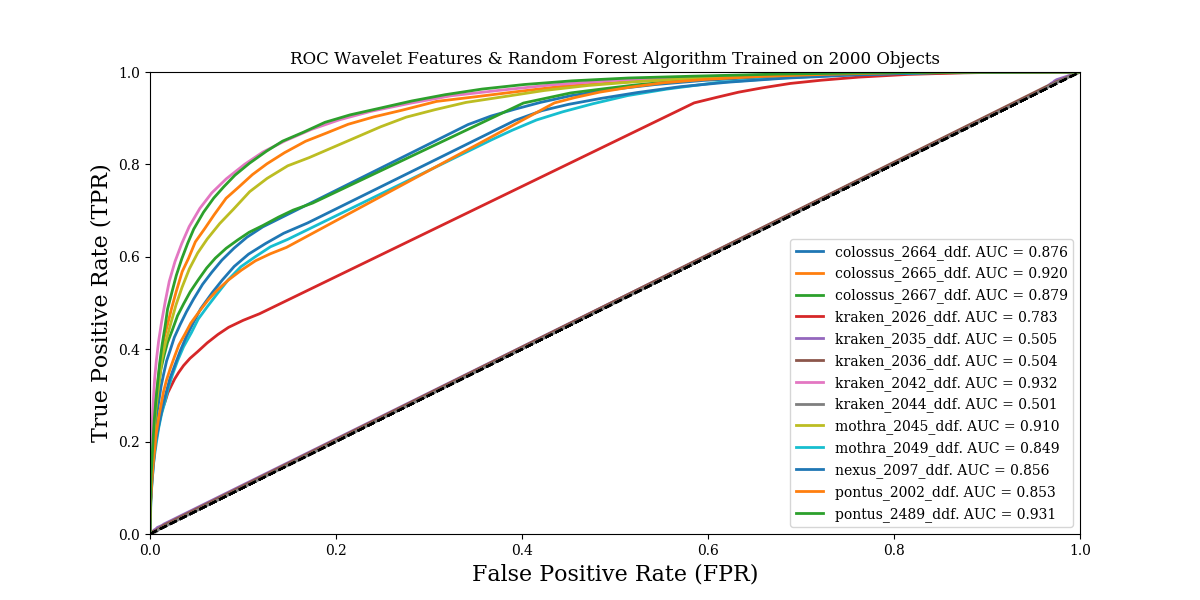
\includegraphics[width=0.8\textwidth]{sn_contrib/Classification_Tarek/figures/photometric_classification_roc_results_ddfY1.png}
        \caption{DDFY1}
        \label{fig:ddfy1}
    \end{subfigure}
    %~ %add desired spacing between images, e. g. ~, \quad, \qquad, \hfill etc.
      %(or a blank line to force the subfigure onto a new line)
    \begin{subfigure}
        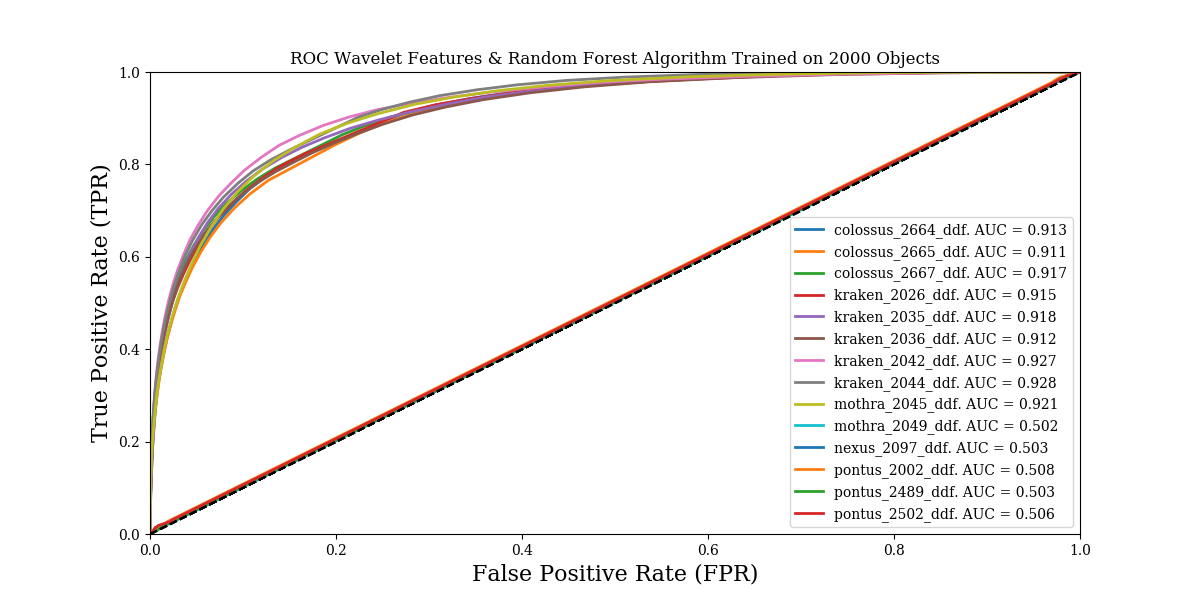
\includegraphics[width=0.8\textwidth]{sn_contrib/Classification_Tarek/figures/photometric_classification_roc_results_ddfY10.png}
        \caption{DDFY10}
        \label{fig:ddfy10}
    \end{subfigure}
   \caption{Comparison for the DDFY1 and DDFY10 ROC curves}\label{fig:rocs}
\end{figure}

Figure\ref{fig:ddfy1} shows the
comparative classification performances between 13 cadences for the Deep
Drilling Fields of Year 1 whereas Figure\ref{fig:ddfy10} compares the same
cadences for the Deep Drilling Fields over the entire survey.

The area under
the Receiver Operating Characteristic (auROC) curves were chosen as the metric
to evaluate the performance. It was felt this single scalar would be most useful
for being able to differentiate the ability of the various cadence strategies
to perform photometric classification.

By interpolating the sampled light curved with Gaussian process and then applying a
wavelet decomposition to these interpolated light curves, one obtains features
that can be provided to a classifier, in this case a Random Forest algorithm.
The performance of the interpolation is directly affected by the amount of
samples one has on the light curve. More samples improves the reliability of the
Gaussian processes and thus provided better features through via the wave decomposition.

Therefore it can be understood that in order to classify transients, short sampling of a light
curve is important. This is particularly important for early classification
leading to possible spectroscopic follow up. Work from Philippe Gris
investigates
the number of \emph{well-sampled} light curves one can obtain from the different
cadence strategies. Separate to that study, analysis of cadence impact on
classification is done here, but nonetheless, a well sampled light curve would
indeed boost classification rate. Thus, before any analysis is conducted, one
could assume a rolling cadence with 2 to 3 days would be beneficial to the
cause.
With this in mind, the results of the analysis shown here do not in particular
point to a specific cadence as be favourable, but the performance of some
strategies do not perform as well as others in the Year 1 case and over the
Year 10 full survey.

This research can be taken further in several ways and there are plans to
continue this analysis for Wide-Fast-Deep cadence runs also. Work is currently
taking place to investigate the performance of classifiers trained on DDF runs
and then tested on WFD. Work is also being carried out for a comparative stufy
of WFD cadence runs much like what has been shown above for DDFY1 and DDFY10.
Further to the two DDF runs presented, further analysis will be carried out for
more years to see the performances for years in between and to see if there
are classification trends that change through the lifetime of the survey. It is
also hoped that number of Supernova used for training affects classification
performances, this work is done but alternations are required to the code for a complete
analysis. Finally it would be beneficial to understand the elements of each cadence
strategy to give further insight as to why certain cadences perform the way they do.

%If the ability to classify
%Supernova is affected in a negative way by a certain cadence then this should be highlighted as
%one that adversely affects the ability to study Type 1a cosmology further.
%Alternatively, if a cadence is shown to give a particularly better rate of
%classification than others, this should be investigated further to determine
%what features result in this outcome, and perhaps could be further optimised.

It is difficult to say at this stage which cadence is preferred until further
analysis is done, and one leaves this to the working group leaders to draw
concrete conclusions.
